% Appendix I -- Full Results of E11-E17 (body). Tables: tables/tabI_*.tex (build/make_tables.py) from
%   tmlr_ext/TD_tdmpc2/results/analysis/td_summary.json, td_e13_cells.csv; DW_dinowm/results/analysis/analysis_dw.json,
%   analysis_posthoc/*.json; MT_317m/results/analysis/e14_eval.csv; K_kernel/results/raw/k.1/analysis*/;
%   coordinator/e17_pc_vs_e12.txt; coordinator/reanalysis/r1_G.csv, r2_fr.csv, r4_pooled.csv, r5_side_by_side.csv;
%   TD_tdmpc2/results/analysis_x5/x5_kstar.csv.
Tables~\ref{tab:overview} and~\ref{tab:components} summarize the damage and the repairs of every family (Sections~\ref{sec:glance} and~\ref{sec:components}). Tables~\ref{tab:e11cells}--\ref{tab:x5} give the cells behind Sections~\ref{sec:break}--\ref{sec:cost}: E11 (every cell), E12 (smallest usable bit widths), E14 (317M), E16 (planner swap), E13 (offline errors on common states), E15 (DMC and iterations), E17 (closed loop of the integer kernel and of pre-converted BF16), the five re-analyses R1--R5 of the E11--E17 results, and the post hoc cell D4 and runs X5, X6 and X17. The re-analyses use no new episodes: R1 bootstraps $k^*$ and $G$ over the paired episodes of each task (stratified for the two-stage cells), R2 varies the damage threshold $\tau$ of $k^*$, R3 counts the bits gained by each dither form alone, R4 pools the two DINO-WM splits with inverse-variance weights, and R5 sets the costs of persistence of both families side by side; all are post hoc. Where a post hoc run overlapped an earlier cell, it reproduced that cell exactly: the E11 \detnoise cells of all \nv{x5.repro.ntasks} Meta-World tasks were reproduced bit for bit on a second machine of the same type.

\begin{table}[h]
\caption{Mean damage over the damaged cells of each group, by rounding variant. E1/E10 are the main stages; E11/E14 re-ran cells on new seeds, and the DINO-WM Wall and PushT columns are the damaged cells of the new split. Meta-World, 317M and DINO-WM in success points, DMC in \% of return; -- not run; $^\dagger$ post hoc cell. Figure~\ref{fig:damage} shows the same cells one by one.}
\label{tab:overview}
\centering\small
\setlength{\tabcolsep}{4pt}
\begin{tabular}{@{}lrrrrrrrrr@{}}
\toprule
 & \multicolumn{2}{c}{5M Meta-World} & \multicolumn{2}{c}{5M DMC} & \multicolumn{2}{c}{317M Meta-World} & \multicolumn{3}{c}{DINO-WM} \\
\cmidrule(lr){2-3}\cmidrule(lr){4-5}\cmidrule(lr){6-7}\cmidrule(lr){8-10}
Variant & E1 & E11 & E1 & E11 & E10 & E14 & E1 & Wall & PushT$^\dagger$ \\
\midrule
\inputrows{tables/tab_overview.tex}
\bottomrule
\end{tabular}
\end{table}

\begin{table}[h]
\caption{Damaged cells repaired ($\red\ge0.5$) by each variant: TD-MPC2 5M (E11, new seeds), 317M (E14) and the two damaged DINO-WM cells of the new split (3 bits; values are $\red$). -- not run; $^\dagger$ post hoc cell.}
\label{tab:components}
\centering\small
\setlength{\tabcolsep}{6pt}
\begin{tabular}{@{}lccccc@{}}
\toprule
Variant & 5M Meta-World & 5M DMC & 317M Meta-World & Wall ($\red$) & PushT$^\dagger$ ($\red$) \\
\midrule
\inputrows{tables/tab_components.tex}
\bottomrule
\end{tabular}
\end{table}

\begin{table}[h]
\caption{E11: every cell. Top: $D_{\dtm}$ in points (\% on DMC), the planned reading of the cell (class), $\dbias=D_{\dtm}-D_{\detbc}$ and $\dpers=D_{\detshiftfix}-D_{\detshift}$, with 95\% intervals. Bottom: $\red$ of each variant.}
\label{tab:e11cells}
\centering\footnotesize
\setlength{\tabcolsep}{4pt}
\begin{tabular}{@{}lrllll@{}}
\toprule
Cell & $k$ & $D_{\dtm}$ & Class & $\dbias$ & $\dpers$ \\
\midrule
\inputrows{tables/tabI_e11_cells.tex}
\bottomrule
\end{tabular}

\medskip
\begin{tabular}{@{}lrccccccc@{}}
\toprule
Cell & $k$ & \detbc & \shep/\shplan & \detshiftfix & \shiterb & \shiter & \detshift & \detnoise \\
\midrule
\inputrows{tables/tabI_e11_red.tex}
\bottomrule
\end{tabular}
\end{table}

\textbf{Checkpoints.} The intervals of the TD-MPC2 stages resample the 90 pairs of a cell and are therefore conditional on its three checkpoints. Table~\ref{tab:e11ckpt} splits every E11 cell by checkpoint (30 pairs each): the damage of \dtm varies considerably between checkpoints, and \shiter repairs most checkpoint-level cells in Meta-World but not on walker and quadruped.

\begin{table}[h]
\caption{E11 by checkpoint (30 pairs each): $D_{\dtm}$ in points (\% of return on DMC) and $\red$ of \shiter; -- where \dtm causes no damage.}
\label{tab:e11ckpt}
\centering\small
\begin{tabular}{@{}lrrrrrrr@{}}
\toprule
 & & \multicolumn{2}{c}{Checkpoint 1} & \multicolumn{2}{c}{Checkpoint 2} & \multicolumn{2}{c}{Checkpoint 3} \\
\cmidrule(lr){3-4}\cmidrule(lr){5-6}\cmidrule(l){7-8}
Task & $k$ & $D_{\dtm}$ & $\red$ & $D_{\dtm}$ & $\red$ & $D_{\dtm}$ & $\red$ \\
\midrule
\inputrows{tables/tabI_e11_ckpt.tex}
\bottomrule
\end{tabular}
\end{table}

\begin{table}[h]
\caption{E12: smallest usable bit width $k^*$ for \dtm / \detbc / \shiter / \detshift, and bits gained $G$, with per-tensor (PT) and per-channel (PC) ranges. DINO-WM has no \detshift arm. $^\ddagger$ borderline; bootstrap in Table~\ref{tab:r1}.}
\label{tab:e12}
\centering\small
\begin{tabular}{@{}lcccc@{}}
\toprule
Task & $k^*$ PT & $G$ PT & $k^*$ PC & $G$ PC \\
\midrule
\inputrows{tables/tabI_e12_kstar.tex}
\bottomrule
\end{tabular}
\end{table}

\begin{table}[h]
\caption{E14 (317M): $D_{\dtm}$ (points), $\red$ of \shiter, the cost of persistence $D_{\shep}-D_{\shiter}$ (points), $r=D_{\shep}/D_{\dtm}$, and $\red$ of \detbc and \detshift.}
\label{tab:e14}
\centering\scriptsize
\setlength{\tabcolsep}{3pt}
\begin{tabular}{@{}lrlllllr@{}}
\toprule
Task & $k$ & $D_{\dtm}$ & $\red$ \shiter & $D_{\shep}-D_{\shiter}$ & $r$ & \detbc & \detshift \\
\midrule
\inputrows{tables/tabI_e14.tex}
\bottomrule
\end{tabular}
\end{table}

\begin{table}[h]
\caption{E16: cost of persistence (TD-MPC2: $D_{\shep}-D_{\shiter}$; DINO-WM: $D_{\shplan}-D_{\shiter}$) with the default and the swapped planner (TD-MPC2: CEM-like, without policy trajectories; DINO-WM: MPPI-like), the damage of \dtm and \shiter with the swapped planner, and the swapped planner's unquantized success relative to the default (qualification: at least 0.6). Points, \% of return on cheetah-run.}
\label{tab:e16}
\centering\scriptsize
\setlength{\tabcolsep}{3.5pt}
\begin{tabular}{@{}llllllr@{}}
\toprule
 & & \multicolumn{2}{c}{Cost of persistence} & \multicolumn{2}{c}{Swapped planner} & \\
\cmidrule(lr){3-4}\cmidrule(lr){5-6}
Model & Task & Default planner & Swapped planner & $D_{\dtm}$ & $D_{\shiter}$ & Relative success \\
\midrule
\inputrows{tables/tabI_e16.tex}
\bottomrule
\end{tabular}
\end{table}

\textbf{Offline errors on common states (E13).} Table~\ref{tab:e13} gives, for each damaged E11 cell, the two sides of the planned comparison Dg1 and the offline errors discussed in Section~\ref{sec:offline} and Appendix~\ref{app:mech}. The mean within-cell difference of the two Spearman correlations is \nv{dg1.mw} on Meta-World (positive in all cells) and \nv{dg1.dmc} on DMC, above the planned threshold of 0.3, and \nv{dg1.dw} in DINO-WM. The persistent share $\rho_p$ is 1 for every fixed variant by construction, which is why the summary statistic nearly restates the manipulated variable.

\begin{table}[h]
\caption{E13 on held-out states common to all variants (TD-MPC2: 90 held-out episodes per task; DINO-WM Wall: 120 states). Dg1: within-cell Spearman correlation of the eight variants' damage with $P_1=\rho_p\cdot\sigma_e/\sigma_J$ (last-iteration candidates) and with $P_2$, the latent one-step error (first-iteration candidates), and their difference (threshold 0.3). Errors of \dtm / \shiter on first-iteration candidates; the reward error is the median absolute error over the candidates' reward standard deviation (DINO-WM: the planning cost). $\rho_p$ on last-iteration candidates.}
\label{tab:e13}
\centering\scriptsize
\setlength{\tabcolsep}{3pt}
\begin{tabular}{@{}lrrrrcccc@{}}
\toprule
 & & \multicolumn{3}{c}{Dg1} & \multicolumn{3}{c}{\dtm / \shiter} & $\rho_p$ \\
\cmidrule(lr){3-5}\cmidrule(lr){6-8}\cmidrule(l){9-9}
Cell & $k$ & $P_1$ & $P_2$ & diff. & latent, 1 step & latent, 5 steps & reward & \detnoise / \shiter / \detshift \\
\midrule
\inputrows{tables/tabI_e13.tex}
\bottomrule
\end{tabular}
\end{table}

\textbf{DMC and planner iterations (E15).} Table~\ref{tab:e15} gives every cell of E15; the unquantized baseline is re-run for every number of iterations. The damage of \dtm stays about the same with more iterations, while that of both dither forms falls on cheetah-run, quadruped-walk and walker-walk, on walker only to about \dtm's level; on finger-turn-hard both forms already repair the damage at six iterations.

\begin{table}[h]
\caption{E15: DMC at the primary bit width with 6, 12 and 24 MPPI iterations (\% of return; 6 iterations = the E11 cells). The last column is the median planning time per control step (ms) of \dtm / \detshift.}
\label{tab:e15}
\centering\scriptsize
\setlength{\tabcolsep}{3.5pt}
\begin{tabular}{@{}lrrrlrrrrc@{}}
\toprule
 & & & & & \multicolumn{2}{c}{\shiter} & \multicolumn{2}{c}{\detshift} & \\
\cmidrule(lr){6-7}\cmidrule(lr){8-9}
Task & Iterations & Pairs & none & $D_{\dtm}$ & $D$ & $\red$ & $D$ & $\red$ & ms \\
\midrule
\inputrows{tables/tabI_e15.tex}
\bottomrule
\end{tabular}
\end{table}

\textbf{Closed loop of the integer path (E17).} Table~\ref{tab:e17} gives K3 for all 12 tasks and K2 for its four tasks; Table~\ref{tab:e17pc} compares the integer configuration with per-channel activation ranges folded into the next layer (int8 weights quantized per output channel) with the fake-quantized per-channel cells of E12. The two come from different machines and are independent samples, so the interval of their difference combines two bootstraps; it contains zero in \nv{e17.pc.n} of \nv{e17.pc.of} cells.

\begin{table}[h]
\caption{E17 closed loop (90 pairs). K3: damage of BF16 with weights converted once in advance (points, \% on DMC). K2: $D_{\dtm}-D_{\detshift}$ with fake quantization (E11) and in the integer kernel.}
\label{tab:e17}
\centering\small
\setlength{\tabcolsep}{4pt}
\begin{tabular}{@{}llll@{}}
\toprule
 & K3 & \multicolumn{2}{c}{K2: $D_{\dtm}-D_{\detshift}$} \\
\cmidrule(l){3-4}
Task & BF16, pre-converted & fake quantization & integer kernel \\
\midrule
\inputrows{tables/tabI_e17.tex}
\bottomrule
\end{tabular}
\end{table}

\begin{table}[h]
\caption{E17: folded per-channel integer configuration against fake quantization with per-channel ranges (E12), damage in points (\% on DMC); $n$ = pairs of the E12 cell (90 for the integer cells).}
\label{tab:e17pc}
\centering\small
\setlength{\tabcolsep}{4pt}
\begin{tabular}{@{}lrllll@{}}
\toprule
Task & $k$ & Variant & Integer & Fake quantization ($n$) & Difference \\
\midrule
\inputrows{tables/tabI_e17pc.tex}
\bottomrule
\end{tabular}
\end{table}

\textbf{Robustness of the bit counts (R1--R3).} Table~\ref{tab:r1} gives, per task and range, the point estimate of $G$ and the bootstrap probabilities that $G\ge1$ and $G\ge2$; Table~\ref{tab:r2} the Meta-World counts behind Fr1 and Fr2 for damage thresholds of 5--20 points and for a strict threshold. With the better dither, both tests hold at every threshold; \shiter alone sits exactly at the count needed at some thresholds.

\begin{table}[h]
\caption{R1 (post hoc): bootstrap of $k^*$ and $G$ over the paired episodes of each task ($10^4$ resamples; better of \shiter and \detshift for TD-MPC2, \shiter for DINO-WM). Point $G$, and the share of resamples with $G\ge1$ and $G\ge2$. RC: rollout-chosen ranges (PushT only).}
\label{tab:r1}
\centering\small
\setlength{\tabcolsep}{4pt}
\begin{tabular}{@{}lccccccccc@{}}
\toprule
 & \multicolumn{3}{c}{PT} & \multicolumn{3}{c}{PC} & \multicolumn{3}{c}{RC} \\
\cmidrule(lr){2-4}\cmidrule(lr){5-7}\cmidrule(l){8-10}
Task & $G$ & $P(G\ge1)$ & $P(G\ge2)$ & $G$ & $P(G\ge1)$ & $P(G\ge2)$ & $G$ & $P(G\ge1)$ & $P(G\ge2)$ \\
\midrule
\inputrows{tables/tabI_r1.tex}
\bottomrule
\end{tabular}
\end{table}

\begin{table}[h]
\caption{R2 (post hoc): number of Meta-World tasks (of 8) that gain at least one bit, for damage thresholds $\tau$ of $k^*$ (points), with the better dither, \shiter alone and \detshift alone, and the number each test needs.}
\label{tab:r2}
\centering\small
\setlength{\tabcolsep}{4pt}
\begin{tabular}{@{}lcccccccc@{}}
\toprule
 & \multicolumn{4}{c}{Fr1 (per tensor)} & \multicolumn{4}{c}{Fr2 (per channel)} \\
\cmidrule(lr){2-5}\cmidrule(l){6-9}
$\tau$ & better & \shiter & \detshift & needed & better & \shiter & \detshift & needed \\
\midrule
\inputrows{tables/tabI_r2.tex}
\bottomrule
\end{tabular}
\end{table}

\textbf{DINO-WM across splits (R4, D4, X17).} Table~\ref{tab:dwsplits} sets each DINO-WM cell of the new split next to E1. The two splits use different evaluation pairs and are therefore unpaired; the new split also ran on another GPU type (RTX 4090 against RTX A5000). Re-running the E1 pairs of PushT at 4 bits on the new GPU type reproduced the E1 damage, and re-running the E1 Wall pairs reproduced the E1 baseline, so the differences come from the splits; X17's episodes agreed with E1 in \nv{x17.agree.det}\% of the \dtm episodes. Pooling the two splits with inverse-variance weights gives \nv{r4.pm3.pooled} points for PointMaze at 3 bits and \nv{r4.wall3.pooled} for Wall at 3 bits. PushT at 4 bits is the only cell whose splits are heterogeneous (heterogeneity test $p=\nv{r4.pusht4.pQ}$, $I^2=\nv{r4.pusht4.i2}\%$; $p=\nv{r4.pusht4.pQ.cluster}$ with the trajectory-level variance of the new split), and it is reported side by side rather than pooled.

\begin{table}[h]
\caption{DINO-WM cells on the E1 split (RTX A5000) and on the new split (RTX 4090): unquantized success (\%), $D_{\dtm}$ (points), the interval of a bootstrap over the new split's trajectories (PushT), the E1 pairs re-run on the new GPU type, and the inverse-variance pooled $D_{\dtm}$ (R4, post hoc). $^\dagger$ post hoc cell (D4).}
\label{tab:dwsplits}
\centering\scriptsize
\setlength{\tabcolsep}{3pt}
\begin{tabular}{@{}lrrlrllrll@{}}
\toprule
 & & \multicolumn{2}{c}{E1 split} & \multicolumn{3}{c}{new split} & \multicolumn{2}{c}{E1 pairs re-run} & \\
\cmidrule(lr){3-4}\cmidrule(lr){5-7}\cmidrule(lr){8-9}
Cell & $k$ & none & $D_{\dtm}$ & none & $D_{\dtm}$ & trajectories & none & $D_{\dtm}$ & Pooled \\
\midrule
\inputrows{tables/tabI_dwsplits.tex}
\bottomrule
\end{tabular}
\end{table}

\textbf{The Wall baseline.} The unquantized model succeeds in \nv{dw.wall3.none}\% of the new Wall pairs against \nv{e1.wall.none}\% of the original ones (\nv{dw.wall.rerun.none}\% when those are re-run on the same machine). Wall's $\dpers=\nv{dw.wall3.dpers}$ points arises because \detshift succeeds \nv{dw.wall3.detshift.better} points more often than the unquantized model, and round-to-nearest at 4 bits also beats the unquantized planner (by \nv{dw.wall4.det.above} points on the new split and \nv{e1.wall4.det.above} on the original pairs), so the unquantized planner is not an upper bound on Wall and $\red$ can exceed 1.

\textbf{Costs of persistence side by side (R5).} Table~\ref{tab:r5} lists, for every DINO-WM contrast of a fixed against a redrawn dither, its estimate and upper bound, and how many TD-MPC2 cells have a lower bound above that upper bound. The families differ in whether the interval excludes zero, not in the size of every cell: several TD-MPC2 cells have lower bounds below some DINO-WM upper bounds.

\begin{table}[h]
\caption{R5 (post hoc): DINO-WM costs of persistence (points) and the number of TD-MPC2 cells whose lower bound of $D_{\shep}-D_{\shiter}$ exceeds the DINO-WM upper bound (5M Meta-World cells of E11, 317M tasks of E14). PushT at 4 bits is outside the planned readings.}
\label{tab:r5}
\centering\small
\setlength{\tabcolsep}{4pt}
\begin{tabular}{@{}lllrrcc@{}}
\toprule
DINO-WM cell & Planner & Contrast & Estimate & Upper & 5M MW & 317M \\
\midrule
\inputrows{tables/tabI_r5.tex}
\bottomrule
\end{tabular}
\end{table}

Figure~\ref{fig:bitspc} shows the Meta-World bit curves with per-channel ranges, in the format of Figure~\ref{fig:bits}.

\begin{figure}[h]
\centering
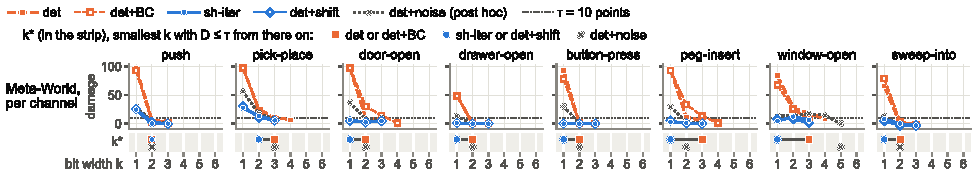
\includegraphics[width=\linewidth]{fig_bitlimit_pc.pdf}
\caption{Damage (success points) against bit width $k$ on Meta-World with per-channel ranges (E12; \detnoise post hoc), as in Figure~\ref{fig:bits}: the dotted line is $\tau=10$ points, missing markers: not run, and the strip under each panel marks the smaller $k^*$ of \dtm and \detbc (square), of \shiter and \detshift (circle) and of \detnoise (cross).}
\label{fig:bitspc}
\end{figure}

\textbf{Fresh noise on the bit axis (X5).} Table~\ref{tab:x5} sets $k^*$ of \detnoise next to the $k^*$ of E12. The E12 values come from another machine of the same type and are not paired with X5, so the comparison is descriptive. The damage of \detnoise is often not monotone in the bit width (per tensor, door-open loses \nv{x5.pt.dooropen3} points at 3 bits but \nv{x5.pt.dooropen2} at 2).

\begin{table}[h]
\caption{X5 (post hoc): smallest usable bit width of \detnoise on Meta-World next to E12's $k^*$ of \dtm / \detbc / \shiter / \detshift, and the bits that \detnoise gains over the better of \dtm and \detbc ($G_{\mathrm{noise}}$).}
\label{tab:x5}
\centering\small
\setlength{\tabcolsep}{4pt}
\begin{tabular}{@{}lcccccc@{}}
\toprule
 & \multicolumn{3}{c}{PT} & \multicolumn{3}{c}{PC} \\
\cmidrule(lr){2-4}\cmidrule(l){5-7}
Task & $k^*$ \detnoise & $k^*$ E12 & $G_{\mathrm{noise}}$ & $k^*$ \detnoise & $k^*$ E12 & $G_{\mathrm{noise}}$ \\
\midrule
\inputrows{tables/tabI_x5.tex}
\bottomrule
\end{tabular}
\end{table}

\textbf{The policy without planning (X6).} Table~\ref{tab:x6} compares TD-MPC2's policy, run without planning, with the unquantized planner on the 90 E11 pairs of each task, and sets it next to the lowest-bit dither configuration of E12 (the smallest $k^*$; among ties, the smaller damage at $k^*$, then per tensor before per channel and \shiter before \detshift). The policy uses the same FP32 encoder and $\pi$ as the planner and never calls the dynamics or reward networks, so it is not quantized; the comparison asks whether the low-bit planner falls below the policy. On Meta-World the policy comes close to the unquantized planner, and the dither configuration is better than the policy in \nv{x6.mw.better} task and the same in \nv{x6.mw.same}; on DMC the policy loses much more, and the dither configuration is better in \nv{x6.dmc.better} of the 4 tasks. Which configuration counts as lowest among ties changes some Meta-World comparisons, so we report these counts only here.

\begin{table}[h]
\caption{X6 (post hoc, D7): TD-MPC2 5M without planning (FP32 policy, mean action) against the unquantized planner (none), 90 pairs: success (\%) on Meta-World, return on DMC, and $D_{\mathrm{policy}}$ (points, \% of return on DMC); next to it the lowest-bit dither configuration of E12 (range, rounding, $k$) and its damage. Better/worse: the two intervals do not overlap; same: they overlap. The DMC cells of E12 have 45 pairs (two-stage cells, intervals not corrected for the interim look).}
\label{tab:x6}
\centering\scriptsize
\setlength{\tabcolsep}{3.5pt}
\begin{tabular}{@{}lrrllrrl@{}}
\toprule
 & & & & \multicolumn{3}{c}{Lowest dither configuration (E12)} & \\
\cmidrule(lr){5-7}
Task & none & policy & $D_{\mathrm{policy}}$ & configuration & $D$ & pairs & vs.\ policy \\
\midrule
\inputrows{tables/tabI_x6.tex}
\bottomrule
\end{tabular}
\end{table}
\clearpage
